\section{Results}
\begin{frame}{Topics}
    \begin{itemize}
        \item 50 words per topic
        \item Multi-lingual
    \end{itemize}
    \visible<2->{
        \begin{table}[H]
        \centering
        \caption{Subset of translated topic IDs and their top 5 descriptive words for the directory-topic concept lattice.}
        \label{tab:dir_topic_topics2terms}
        \resizebox{\textwidth}{!}{%
            \begin{tabular}{|
                    >{\columncolor[HTML]{D4D4D4}}l |l|l|l|l|l|}
                \hline
                \rowcolor[HTML]{D4D4D4}
                \textbf{Topic ID} & \multicolumn{5}{c|}{\textbf{Topic Words}}                                                                   \\ \hline
                \textbf{34}       & gun                                       & weapons      & rifles          & pistol         & firearm       \\ \hline
                \textbf{36}       & terminological                            & nonverbal    & linguist        & codeword       & longtext      \\ \hline
                \textbf{54}       & microelectron                             & microkernels & microparticle   & microphysics   & microcosmic   \\ \hline
                \textbf{56}       & pythonpath                                & pythonmac    & python\_version & python\_object & pythonpowered \\ \hline
                \textbf{58}       & nuclear                                   & hazardous    & explosive       & nanotoxicity   & chernobyl     \\ \hline
                \textbf{94}       & project                                   & fundraiser   & donation        & volunteering   & charity       \\ \hline
            \end{tabular}%
            }
        \end{table}
        }
\end{frame}

\begin{frame}{Directory-Topic Concept Lattice}

    \begin{figure}[t]
        \centering
        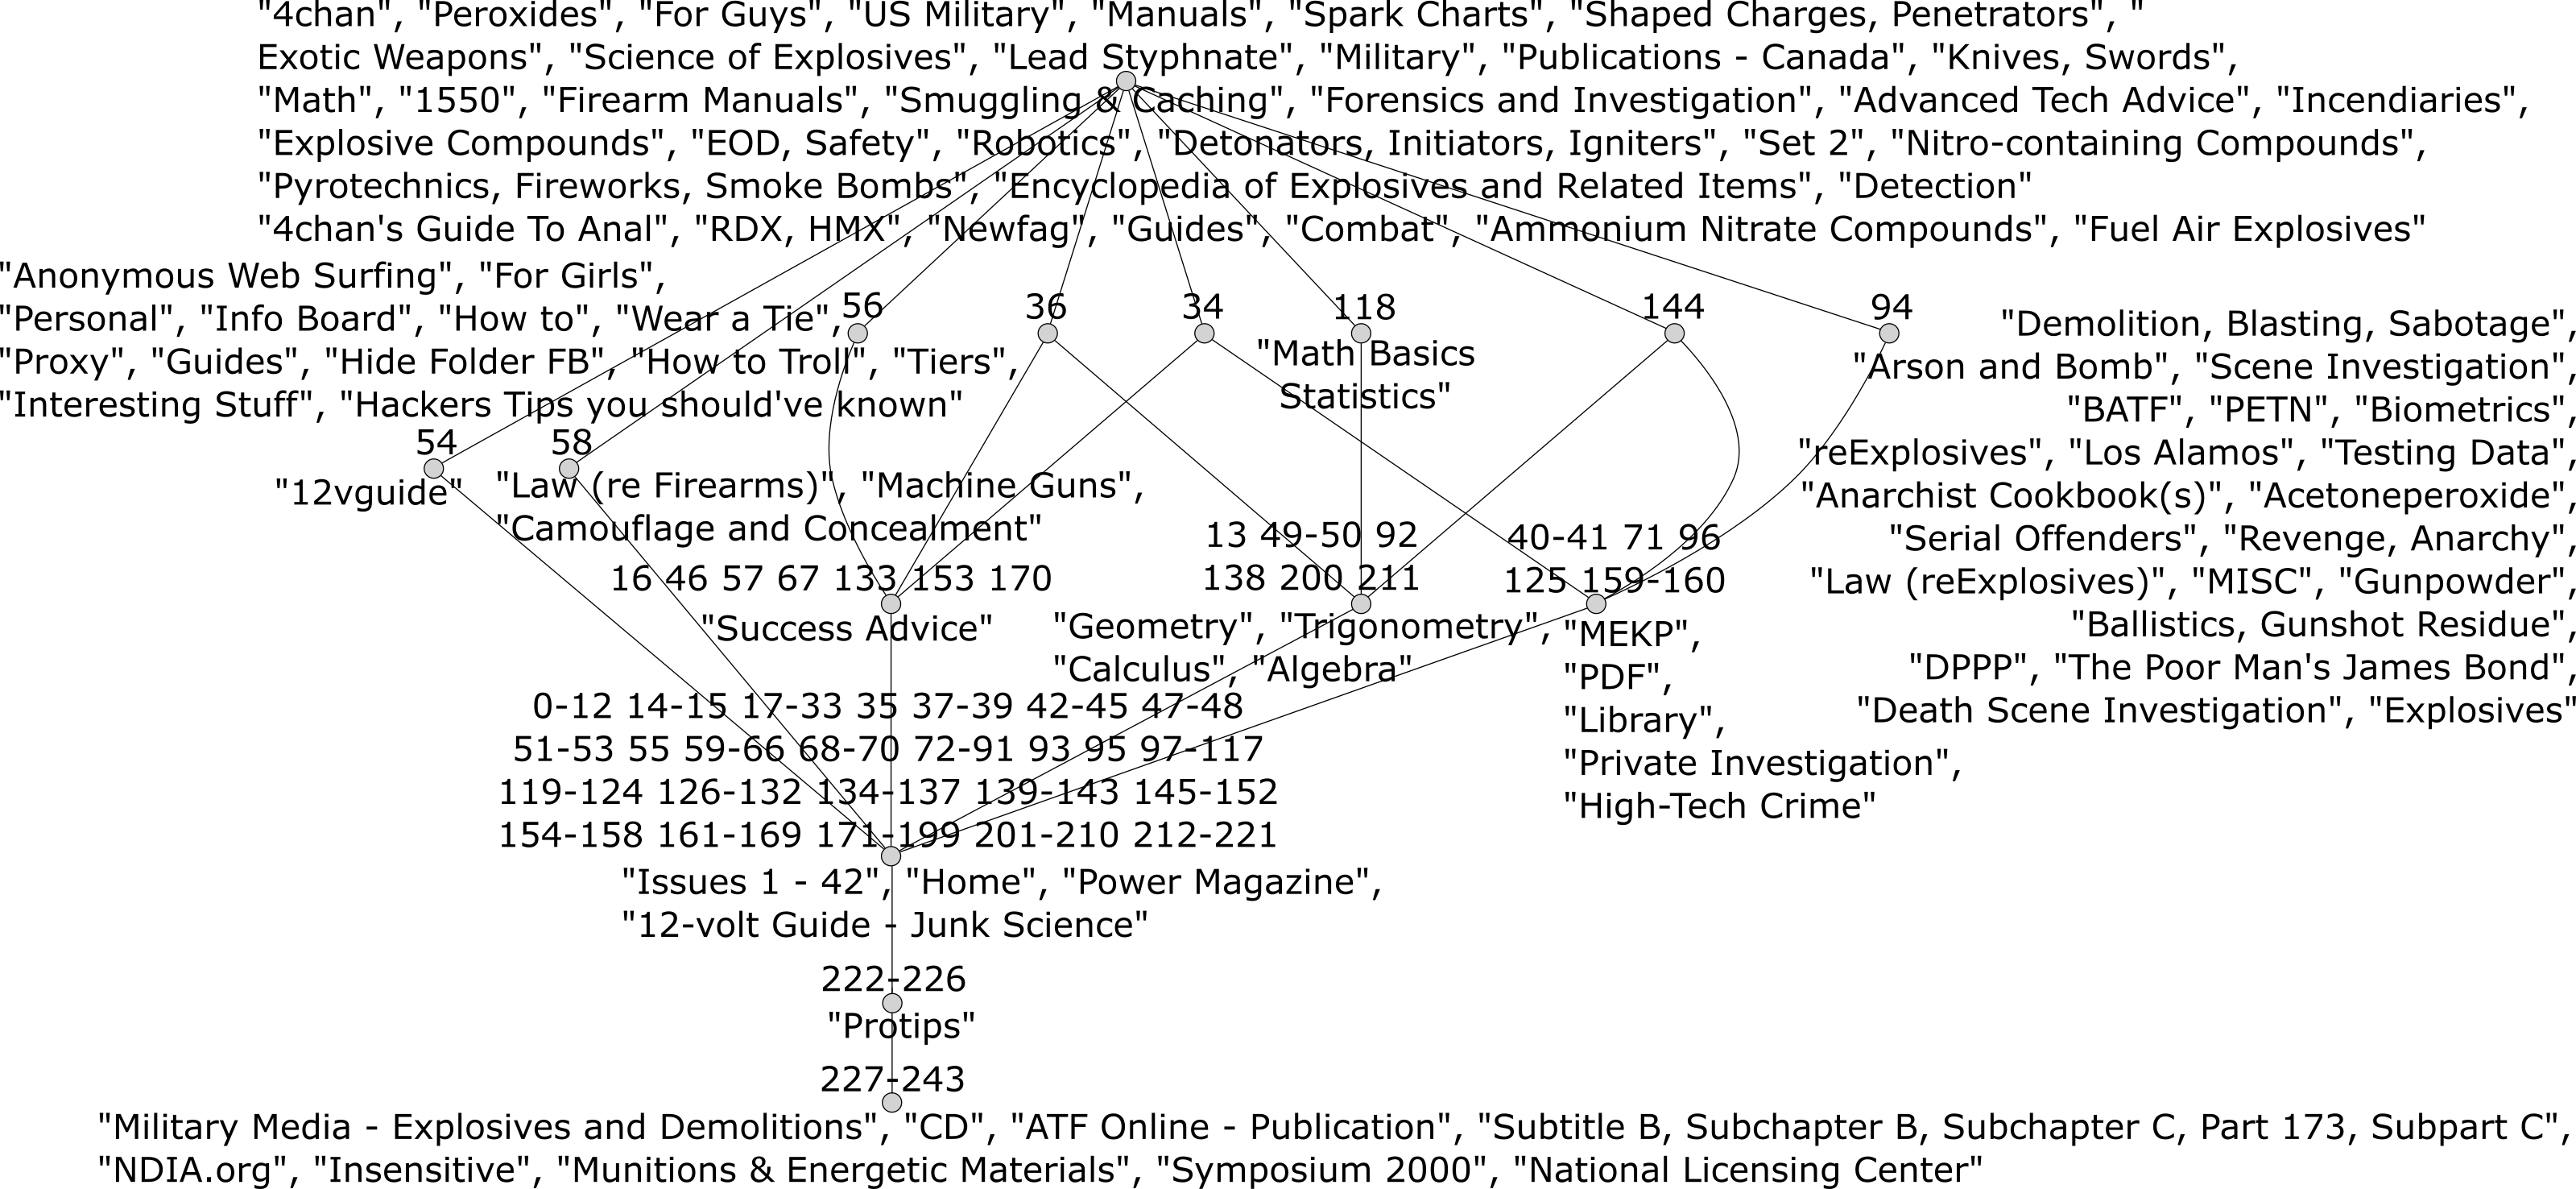
\includegraphics[width=\textwidth]{images/fca_graph_across_dirs_02_03_25_altered3.png}
        \caption{\ac{dataset} directory-topic concept lattice.
            The text entries below the nodes represent directory names, number above nodes denote topic IDs.
        }
        \label{fig:fca_across_dirs}
    \end{figure}
    
\end{frame}

\begin{frame}{Directory-Topic Concept Lattice}

    \begin{itemize}
        \item "Common to specific": Topics propagate downwards 
        \item<2-> Motifs
        \item<3-> Majority of bottom nodes is subdirectory
        \item<4-> Lower nodes introduce philosophical topics
    \end{itemize}

    \visible<2->{
        \begin{definition}
            A motif is a statistically significant subgraph or pattern \cite{hirth_ordinal_2024}.
        \end{definition}
    }
\end{frame}